\documentclass[twocolumn]{article}
\usepackage{url}
\usepackage{titling}
\usepackage{graphicx}
\usepackage{hyperref}
\usepackage[utf8]{inputenc}
\usepackage{array,etoolbox}
\usepackage[none]{hyphenat}
\usepackage[justification=centering]{caption}
\usepackage[acronym,nomain,nonumberlist,nogroupskip,nopostdot]{glossaries}

% loads the list of abbreviations
\makeglossaries
\loadglsentries{acronym}

% centers the title page
\renewcommand\maketitlehookd{\vfill\null}
\renewcommand\maketitlehooka{\null\mbox{}\vfill}

% keywords command
\providecommand{\keywords}[1]
{
  \small
  \noindent \textbf{\textit{Keywords ---}} #1
}

% counter for table
\preto\tabular{\setcounter{magicrownumbers}{0}}
\newcounter{magicrownumbers}
\newcommand\rownumber{\stepcounter{magicrownumbers}\arabic{magicrownumbers}}


\title{\gls{asl}\\
	Fingerspelling Detection}
\author{Shoaib Mohammed}
\date{01 June 2021}


\begin{document}

\begin{titlingpage}
\maketitle
\end{titlingpage}

\begin{abstract}
Approximately 70 million people around the world are deaf-mute. While 
translation services have become easily accessible for about 100 
languages, sign language is still an area that has not been explored. 
Our goal is to detect \& translate the letters of \gls{asl} in real-time.
\end{abstract}

\keywords{\gls{asl}, fingerspelling, \gls{cnn}, transfer learning, 
computer vision}


\section{Introduction}

\subsection{Background}
According to the \gls{csd} \cite{csd}, there are 360 million deaf people 
worldwide. Another report by the \gls{who} \cite{who} bumps up the number to 
466 million people or over 6\% of the world's population suffering from 
disabling hearing loss. But even in this age of technology and communication, 
we are yet to see a universal translation system that helps bridge the gap 
between people that can and cannot speak. \gls{asl} is a natural language 
meaning it was not created and was spread by the people who employ the signs 
by the movement of hands, facial expressions, and body posture. The goal of 
this project is to detect and accurately translate the letters in \gls{asl}.

% (TODO: cite image to the website https://qualityansweringservice.com/american-sign-language-guide/)
\begin{figure}[h]
\centering
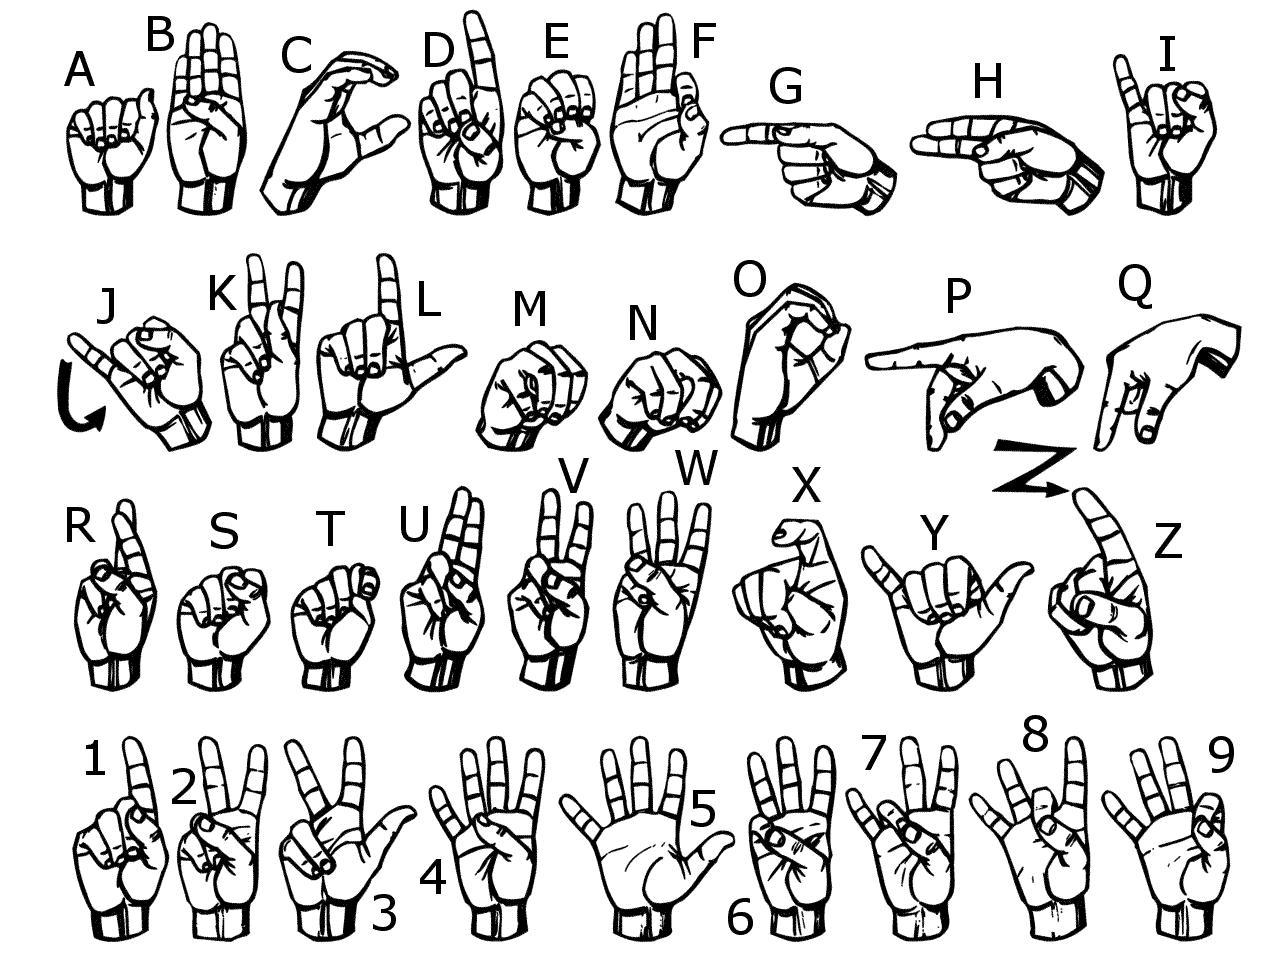
\includegraphics[width=8cm]{./figures/asl alphabets}
\caption{Alphabets in \gls{asl}}
\label{asl alphabets}
\end{figure}

\subsection{Geographical Distribution}

The true count for the number of sign languages is still unknown given the 
vast majority, however, \textit{Ethnologue} \cite{ethnologue} lists this 
number to be \textit{137} \cite{fenlon2015sign}. Given the vast majority, 
\gls{asl} is still the most popular sign language and is being widely used 
around the globe. In addition to being the primary source of communication for 
a sign language in the United States, \gls{asl} is being used throughout most 
of the provinces in Canada \cite{al2010sign}.

\begin{figure}[h]
\centering
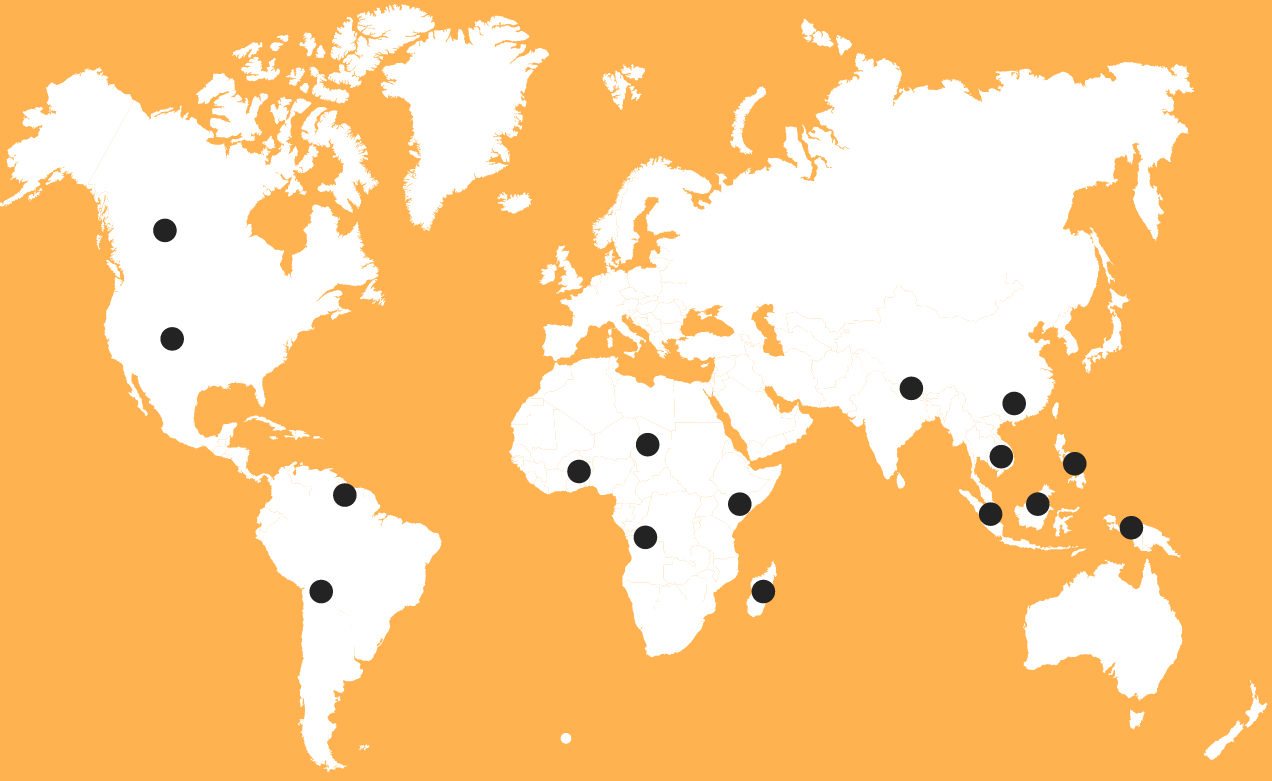
\includegraphics[width=8cm]{./figures/asl being used around the world}
\caption{ASL being used around the world}
\end{figure}

Variations of \gls{asl} are also being used worldwide. Sign language 
similar to \gls{asl} is being used throughout Africa in places such as 
Nigeria, Ghana, Guyana, Central African Republic, Jamaica, Zimbabwe, and 
Kenya \cite{nyst2010sign}.

\subsection{Scope \& Limitations}

% (TODO: do we want to add acronyms for US & UK?)
The bottom line is that there is no universal sign language. For instance, the 
\gls{bsl} differs by a great margin from \gls{asl}, this is clear when 
comparing \autoref{asl alphabets} with \autoref{bsl alphabets}. Generally 
speaking, a person in the US can understand spoken English in the UK but this 
is not the case with sign language. Even though there is a multitude of sign 
languages being used across the world, if an accurate model was developed to 
recognize a sign language, in our case, \gls{asl}, the same methodology could 
be applied to recognize other sign languages.

% (TODO: cite image to the website https://universeofmemory.com/british-sign-language-resources/)
\begin{figure}[h]
\centering
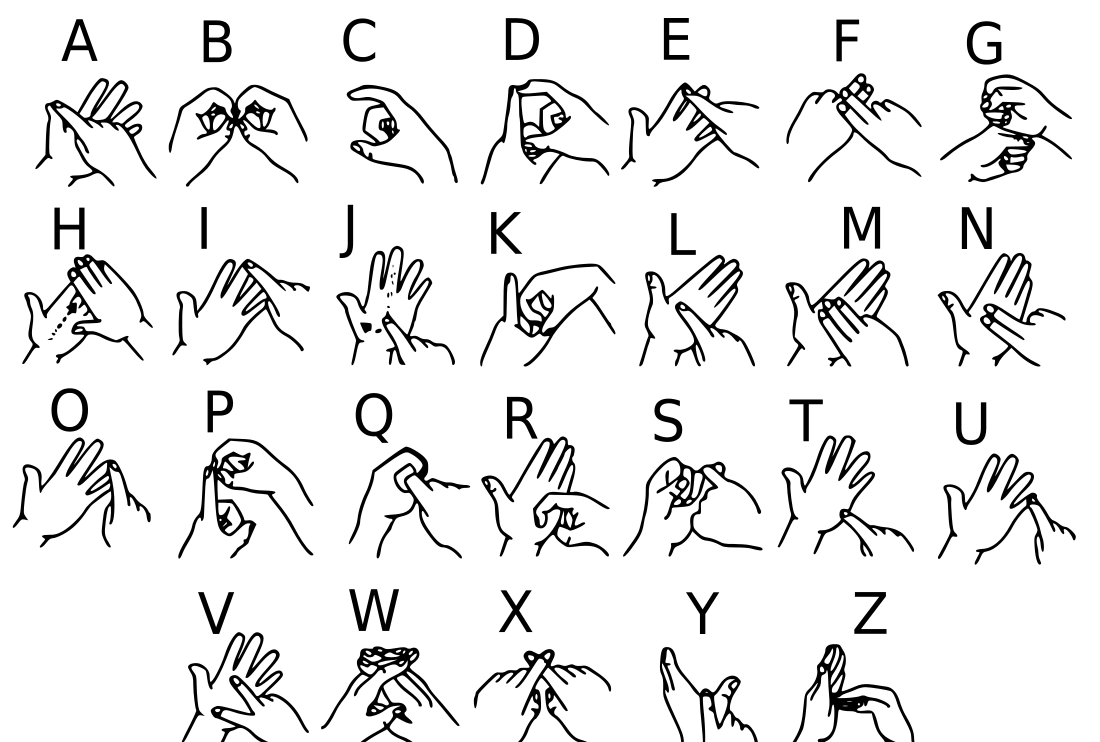
\includegraphics[width=8cm]{./figures/bsl alphabets}
\caption{Alphabets in \gls{bsl}}
\label{bsl alphabets}
\end{figure}

One big limitation for classification is that most signs require motion and 
are not static. Even more so as there are signs which are formed by the same 
motion but the repetition or the number of times a motion is repeated differs. 
Things get even more challenging as facial expressions are important in sign 
languages which is akin to the vocal tone of a person's voice when speaking. 
Two signs may be exactly the same visually but the face gesture of the signer 
makes them different.

Perhaps the major limitation is classifying each sign from the sheer corpus of 
signs in \gls{asl}. A dictionary on \gls{asl} contains illustrations for more 
than \textit{1,600} signs \cite{tennant1998american}. However, our focus is 
classifying the alphabets alone which limits our range to \textbf{24} 
alphabets since we exclude the alphabets J \& Z because these require motion.

\section{Literature Survey}

\subsection{Population Statistics}
A combined study in \cite{mitchell2006many} estimates there were more than 
250,000 deaf people and as many as 500,000 people who used \gls{asl} in 1972. 
Over the years, this number has been on the rise. Based on their research for 
in year 2006, fewer than 1 in 20 Americans or 10,000,000 people suffered from 
\textit{hard of hearing} and close to 1,000,000 were classified as 
\textit{functionally deaf}.

\begin{figure}[h]
\centering
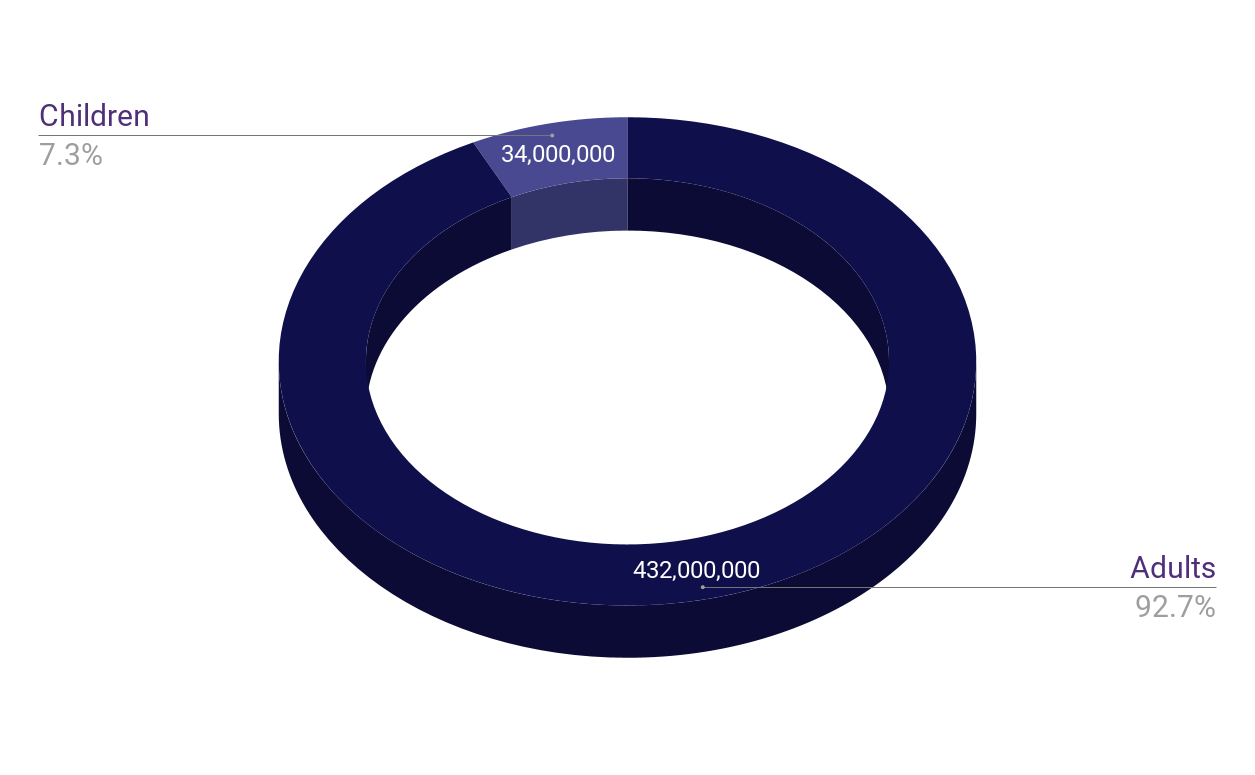
\includegraphics[width=8cm]{./figures/distribution of the population}
\caption{Distribution of the population}
\end{figure}

In 2016, the \gls{nidcd} \cite{nidcd} released statistics about hearing loss 
in the United States. About 2 to 3 out of every 1,000 children have hearing 
loss. Approximately 15\% of adults (37.5 million) aged 18 and over report 
trouble hearing and 18\% of adults aged 20-69 have speech-frequency hearing 
loss in both ears. Furthermore, about 2\% of adults aged 45-54, 8.5\% of 
adults aged 55-64, 25\% of adults aged 65-74, and 5\% of adults aged 75 and 
older have disabling hearing loss.

In terms of the distribution of people suffering from hearing loss \cite{who}, 
432 million people are adults and 34 million are children. Future projections 
estimate 630 million people by 2030 and over 900 million people by 2050.

\subsection{Existing Models}

There has been ongoing research in this area with the growth in machine 
learning and datasets being made available publicly. Many of the models use 
Kinect to recognize the hand gestures and map them to \gls{asl}.

Earlier versions of work used a sensory glove. In 2005, Cemil and Ming 
\cite{oz2005recognition} worked on recognizing the alphabets in \gls{asl} by 
using a sensory Cyberglove and a motion tracker to extract the gestures. By 
processing the data of the fingers on the strain gauges, the trajectory, and 
orientation from the motion tracker through an \gls{ann}, high accuracy 
results were achieved. Building upon this in 2011, Cemil and Ming 
\cite{oz2011american} used feature extraction with noise reduction and were 
able to classify 50 ASL words. A similar approach was used in 2014 
\cite{patil2014american} where the output of the sensor glove gets sent to a 
microcontroller through an \gls{adc}. The glove uses flex sensors which 
capture the bending of each finger. The predicted letter gets displayed on an 
LCD. Although this worked well, it is impractical in real-life. The whole 
system requires several high components to be connected each time someone 
needs to sign a letter.

% (TODO: cite image to the website http://www.cyberglovesystems.com/)
\begin{figure}[h]
\centering
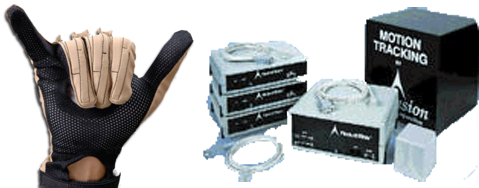
\includegraphics[width=8cm]{./figures/cyberglove and flock of birds}
\caption{Cyberglove and Flock of Birds by Ascension}
\end{figure}

Due to the sophisticated components required by using sensor gloves, there's 
been lots of research on translating ASL by using depth cameras. In 2015, we 
had a major breakthrough successfully translating the 24 static \gls{asl} 
alphabet signs using a Microsoft Kinect \cite{dong2015american}. A latex 
color glove allowed for easier hand segmentation and localizing the joint 
positions. The prediction was done through a \gls{rf} classifier on the depth 
data. The Kinect has also been used in conjunction with hidden Markov 
models \cite{lang2012sign} for recognition. Even with good results, the Kinect 
is not something people just carry around. Furthermore, depth cameras are also 
known to perform badly under poor lighting conditions.

% (TODO: cite image to the reference \cite{dong2015american}
% paper https://openaccess.thecvf.com/content_cvpr_workshops_2015/W15/papers/Dong_American_Sign_Language_2015_CVPR_paper.pdf)
\begin{figure}[h]
\centering
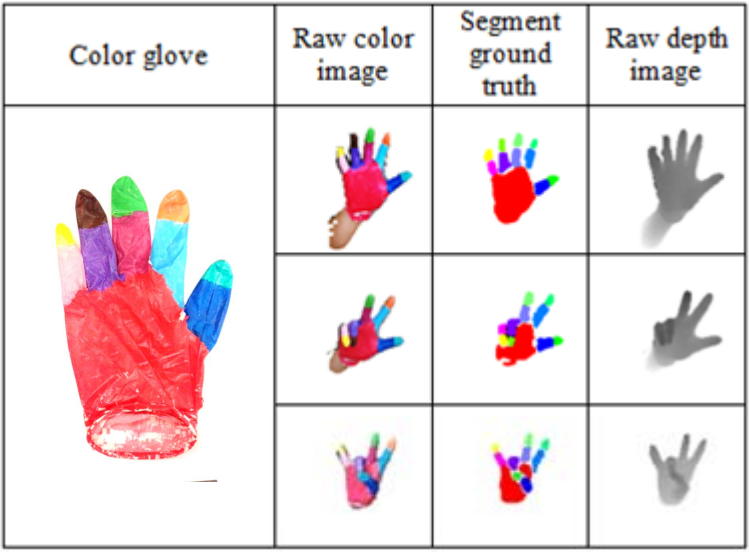
\includegraphics[width=8cm]{./figures/color glove}
\caption{A color glove allowed easier hand segmentation}
\end{figure}

In 2015, a hand gesture recognition model was developed using depth and 
intensity channels with 3D \gls{cnn} \cite{molchanov2015hand}. A similar 
methodology was used to recognize sign language by extracting spatio-temporal 
features \cite{huang2015sign}. To improve the performance, multi-channels of 
video streams including color, depth, and body joint information are used as 
input to the 3D \gls{cnn}. In 2017, a features extractor with deep behavior 
was used to deal with the Arabic Sign Language \cite{elbadawy2017arabic}. By 
combining the features extractor with a 3D \gls{cnn}, the recognition system 
was fed with data from depth maps and could recognize 25 gestures.

% (TODO: cite image to the reference paper "Explaining hyperspectral imaging based plant disease identification: 3D CNN and saliency maps"
% paper https://www.researchgate.net/publication/324744613_Explaining_hyperspectral_imaging_based_plant_disease_identification_3D_CNN_and_saliency_maps)
\begin{figure}[h]
\centering
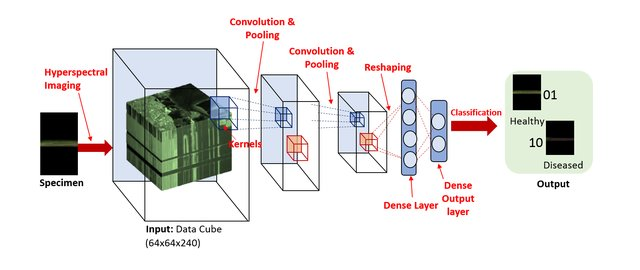
\includegraphics[width=8cm]{./figures/3d cnn}
\caption{3D Convolutional Neural Network}
\end{figure}

In 2018 a different solution was proposed, SignFi \cite{ma2018signfi} which 
uses Wi-Fi to recognize sign language. SignFi can recognize 276 gestures 
involving the head, arm, hand, and finger gestures with high accuracy. SignFi 
works based on \gls{csi} which describes how a signal propagates from the 
transmitter to the receiver at a certain carrier frequency. SignFi uses Wi-Fi 
packets as input and a 9-layer \gls{cnn} as the classification algorithm.

Realizing the challenges faced by the above mentioned methods, our goal is to 
create a machine learning model with transfer learning to classify the 
alphabets of \gls{asl} in real-time. By using \textit{four} transfer learning 
models, namely, MobileNetV2 \cite{sandler2018mobilenetv2}, 
Xception \cite{chollet2017xception}, Inceptionv3 \cite{szegedy2016rethinking}, 
and Inception-ResNetv2 \cite{szegedy2017inception}, we achieve a high accuracy.


\bibliographystyle{ieeetr}
\bibliography{biblio}

\listoffigures
\listoftables

\glsaddall
\setlength{\glsdescwidth}{0.8\textwidth}
\printglossary[type=\acronymtype,title=List Of Abbreviations]

% (TODO: use a clearer way to separate)
\clearpage
\LARGE{\textbf{Additional Resources}}

% (TODO: cite image to the website https://www.javatpoint.com/serialization-in-java)
\begin{figure}[h]
\centering
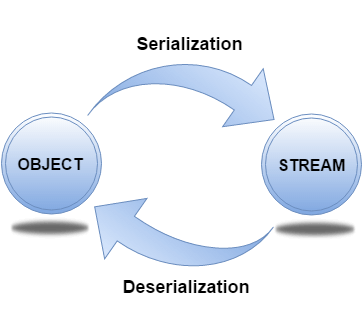
\includegraphics[width=8cm]{./figures/serialization and deserialization}
\caption{Process of serialization \& deserialization}
\end{figure}

\begin{figure}[h]
\centering
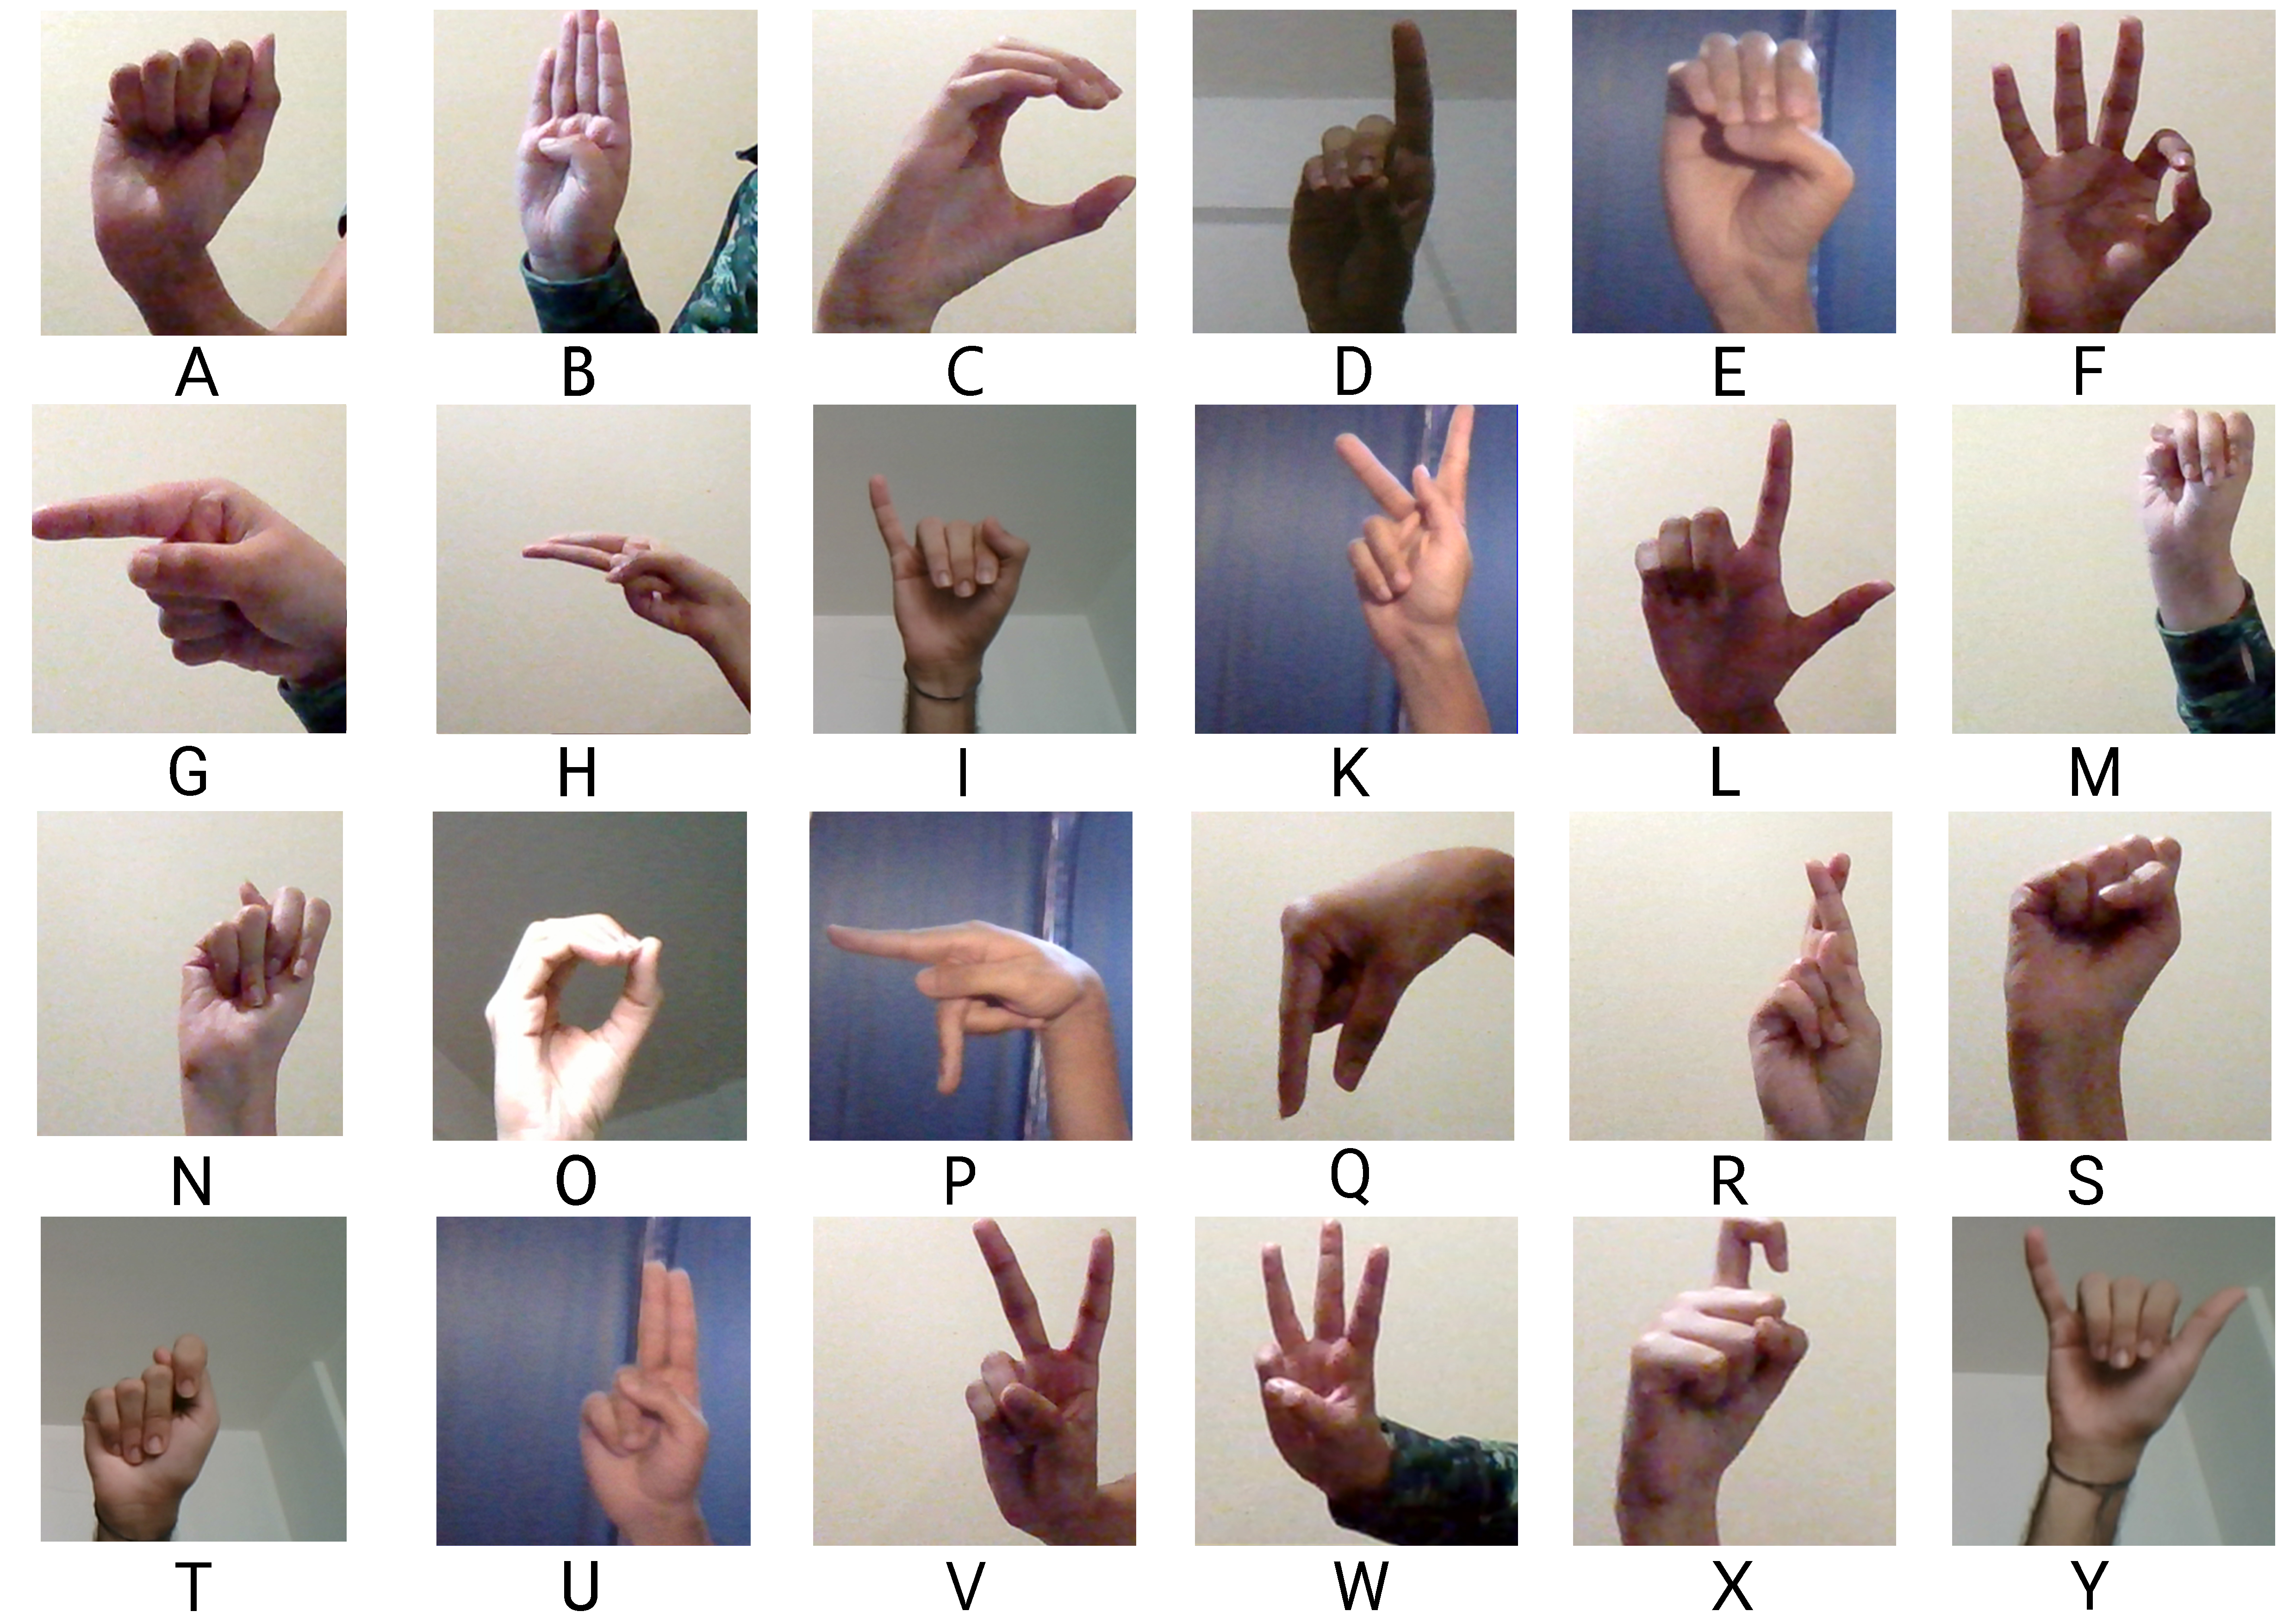
\includegraphics[width=8cm]{./figures/alphabets}
\caption{ASL alphabets from our dataset}
\end{figure}

% (TODO: cite image to the website https://medium.datadriveninvestor.com/introducing-transfer-learning-as-your-next-engine-to-drive-future-innovations-5e81a15bb567)
\begin{figure}[h]
\centering
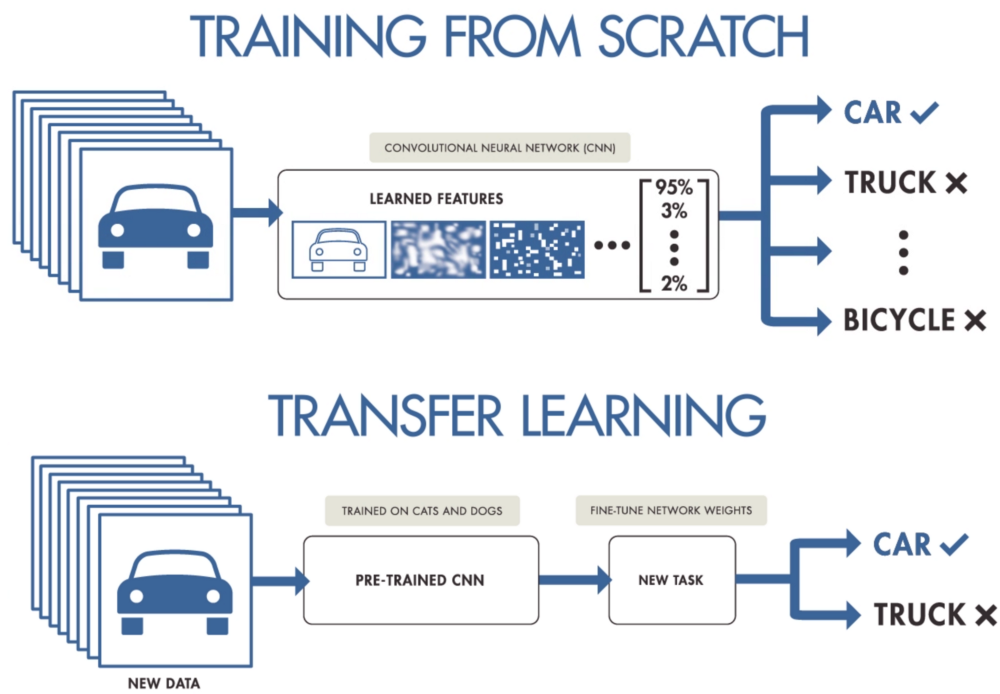
\includegraphics[width=8cm]{./figures/training from scratch vs. transfer learning}
\caption{Training from scratch vs. transfer learning}
\end{figure}

% (TODO: cite image to the website https://medium.com/@lorenzofamiglini/transfer-learning-with-deep-learning-machine-learning-techniques-b4052befe7e2)
\begin{figure}[h]
\centering
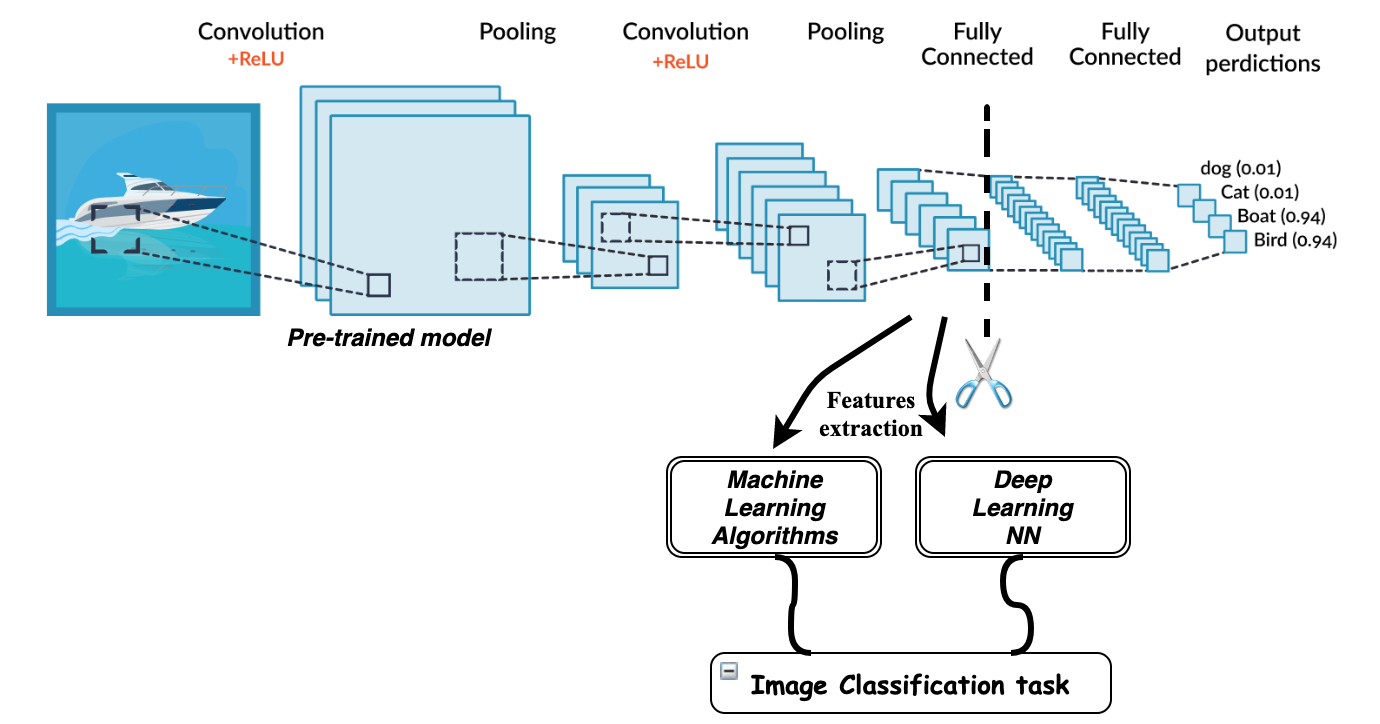
\includegraphics[width=8cm]{./figures/transfer learning process}
\caption{Transfer learning process}
\end{figure}

% (TODO: cite image to the website https://www.quora.com/What-is-the-benefit-of-using-average-pooling-rather-than-max-pooling)
\begin{figure}[h]
\centering
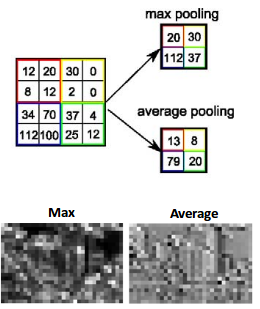
\includegraphics[width=8cm]{./figures/max pooling vs. average pooling}
\caption{Max pooling vs. Average pooling}
\end{figure}

% (TODO: cite image to the website https://medium.com/analytics-vidhya/understanding-a-single-neurons-role-in-neural-network-77bb3251e9db)
\begin{figure}[h]
\centering
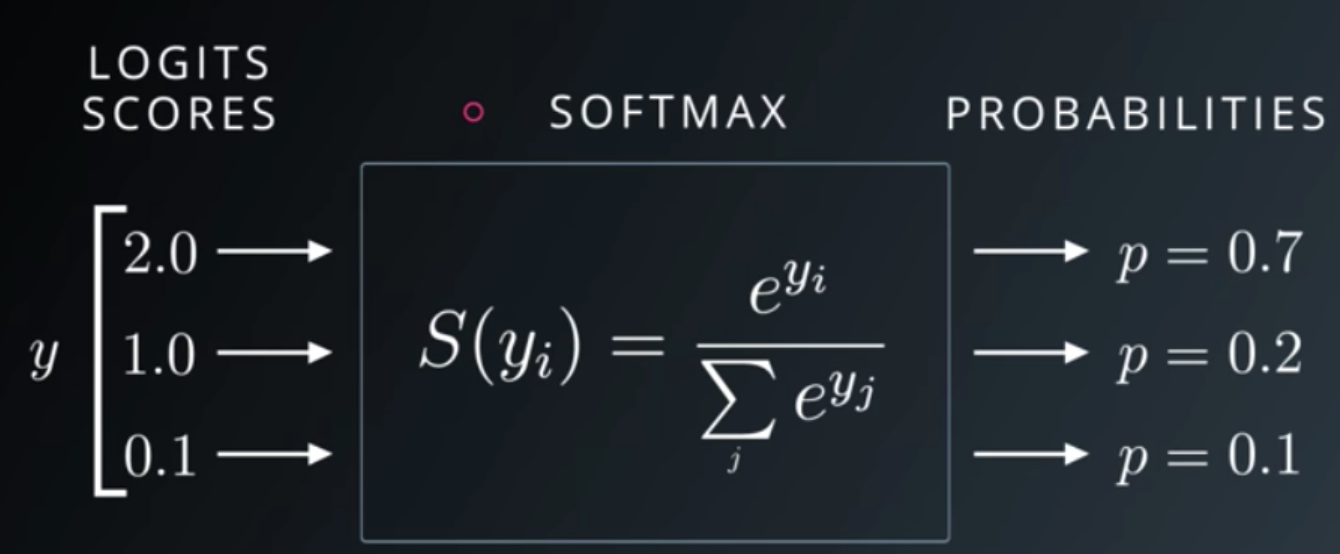
\includegraphics[width=8cm]{./figures/softmax function}
\caption{Softmax function pushing high scores close to 1 and low scores close to 0}
\end{figure}

\begin{figure}[h]
\centering
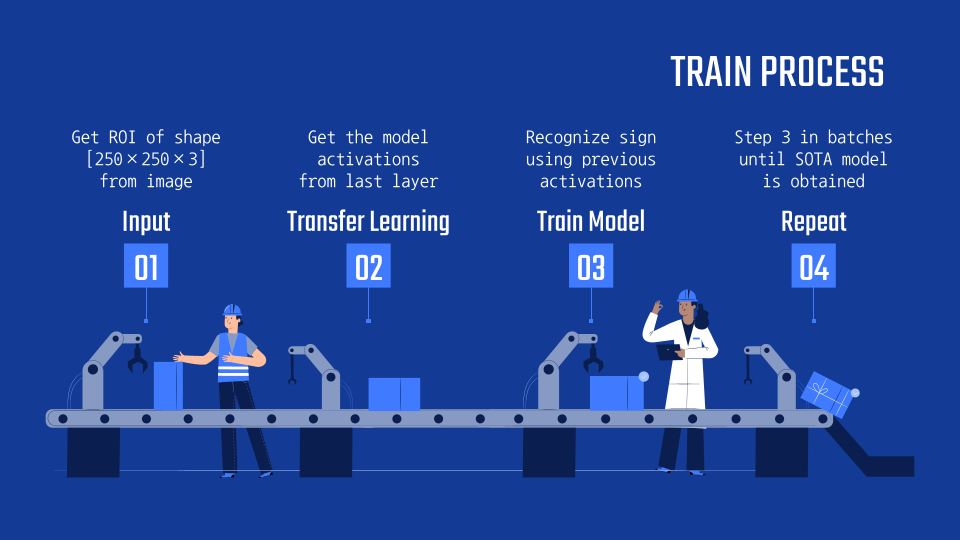
\includegraphics[width=8cm]{./figures/train process}
\caption{Process of training the model}
\end{figure}

\begin{figure}[h]
\centering
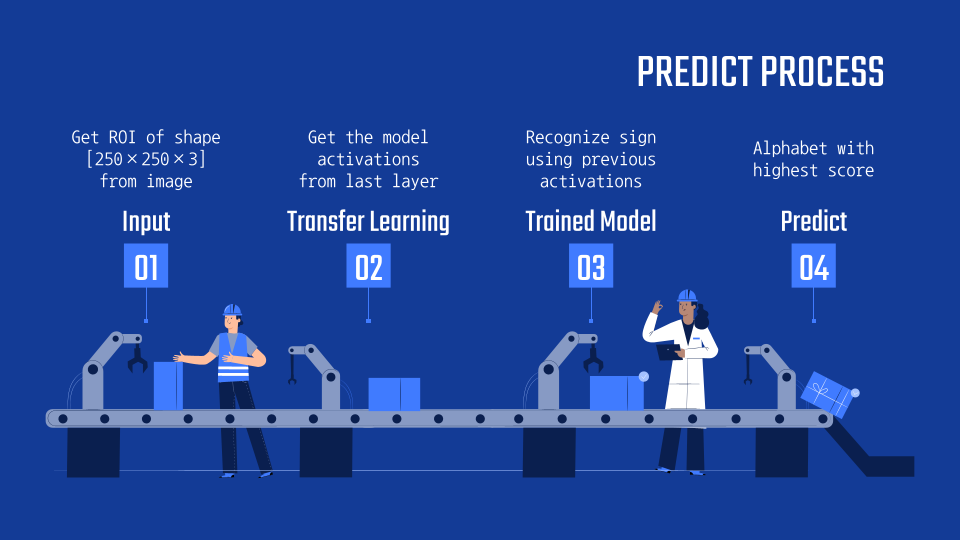
\includegraphics[width=8cm]{./figures/predict process}
\caption{Process of testing the model}
\end{figure}

% (TODO: use a clearer way to separate)
\clearpage

\begin{table}[h]
\begin{tabular}{ |l|c|c|c| }
  \hline
  \textbf{Model} & \textbf{Size} & \textbf{Accuracy} & \textbf{Parameters} \\ \hline
  MobileNetV2 & 14 MB & 0.713 & 3,538,984 \\ \hline
  InceptionV3 & 92 MB & 0.779 & 23,851,784 \\ \hline
  Xception & 88 MB & 0.790 & 22,910,480 \\ \hline
  InceptionResNetV2 & 215 MB & 0.803 & 55,873,736 \\
  \hline
\end{tabular}
\caption{Transfer learning model statistics}
\end{table}

\begin{table}[h]
\begin{tabular}{ |l|c|c|c| }
  \hline
  \textbf{Model} & \textbf{Size} & \textbf{Accuracy} & \textbf{Parameters} \\ \hline
  MobileNetV2 & 91 MB & 0.918 & 7,934,872 \\ \hline
  InceptionV3 & 99 MB & 0.924 & 8,598,424 \\ \hline
  Xception & 100 MB & 0.908 & 8,721,304 \\ \hline
  InceptionResNetV2 & 93 MB & 0.848 & 8,074,136 \\
  \hline
\end{tabular}
\caption{Trained model statistics using varying transfer learning models}
\end{table}

% (TODO: use a clearer way to separate)
\clearpage

\begin{table}[h]
\begin{tabular}{ | @{\makebox[2em][r]{\rownumber\space}} |l|c| }
  \hline
  \multicolumn{1}{ | @{\makebox[2em][r]{\textbf{ ID }}} |l| }{\textbf{Layer (Type)}} 
  & \multicolumn{1}{ |c| }{\textbf{Number of Parameters}} \\ \hline
  \texttt{dense\_1 (Dense)} & \emph{dependent} \\ \hline
  \texttt{dense\_2 (Dense)} & 524,800 \\ \hline
  \texttt{dense\_3 (Dense)} & 131,328 \\ \hline
  \texttt{dense\_4 (Dense)} & 32,896 \\ \hline
  \texttt{up\_sampling2d\_1 (UpSampling2D)} & 0 \\ \hline
  \texttt{conv2d\_5 (Conv2D)} & 131,136 \\ \hline
  \texttt{depthwise\_conv2d\_1 (DepthwiseConv2D)} & 1,088 \\ \hline
  \texttt{up\_sampling2d\_2 (UpSampling2D)} & 0 \\ \hline
  \texttt{depthwise\_conv2d\_2 (DepthwiseConv2D)} & 1,088 \\ \hline
  \texttt{conv2d\_6 (Conv2D)} & 65,600 \\ \hline
  \texttt{dense\_5 (Dense)} & 8,320 \\ \hline
  \texttt{dense\_6 (Dense)} & 33,024 \\ \hline
  \texttt{dense\_7 (Dense)} & 131,584 \\ \hline
  \texttt{dense\_8 (Dense)} & 525,312 \\ \hline
  \texttt{dense\_9 (Dense)} & 2,099,200 \\ \hline
  \texttt{dense\_10 (Dense)} & 2,098,176 \\ \hline
  \texttt{dense\_11 (Dense)} & 524,800 \\ \hline
  \texttt{dense\_12 (Dense)} & 131,328 \\ \hline
  \texttt{dense\_13 (Dense)} & 32,896 \\ \hline
  \texttt{max\_pooling2d\_1 (MaxPooling2D)} & 0 \\ \hline
  \texttt{flatten\_1 (Flatten)} & 0 \\ \hline
  \texttt{dense\_14 (Dense)} & \emph{dependent} \\
  \hline
\end{tabular}
\caption{Model architecture and number of parameters in each layer}
\end{table}

% (TODO: use a clearer way to separate)
\clearpage

\begin{table}[h]
\begin{tabular}{ | @{\makebox[2em][r]{\rownumber\space}} |l|l| }
  \hline
  \multicolumn{1}{ | @{\makebox[2em][r]{\textbf{ ID }}} |l| }{\textbf{Layer (Type)}}
  & \multicolumn{1}{ |c| }{\textbf{Number of Parameters}} \\ \hline
  \texttt{(None, 8, 8, 1024)} & \texttt{(None, 6, 6, 1024)} \\ \hline
  \texttt{(None, 8, 8, 512)} & \texttt{(None, 6, 6, 512)} \\ \hline
  \texttt{(None, 8, 8, 256)} & \texttt{(None, 6, 6, 256)} \\ \hline
  \texttt{(None, 8, 8, 128)} & \texttt{(None, 6, 6, 128)} \\ \hline
  \texttt{(None, 16, 16, 128)} & \texttt{(None, 12, 12, 128)} \\ \hline
  \texttt{(None, 13, 13, 64)} & \texttt{(None, 9, 9, 64)} \\ \hline
  \texttt{(None, 10, 10, 64)} & \texttt{(None, 6, 6, 64)} \\ \hline
  \texttt{(None, 20, 20, 64)} & \texttt{(None, 12, 12, 64)} \\ \hline
  \texttt{(None, 17, 17, 64)} & \texttt{(None, 9, 9, 64)} \\ \hline
  \texttt{(None, 14, 14, 64)} & \texttt{(None, 6, 6, 64)} \\ \hline
  \texttt{(None, 14, 14, 128)} & \texttt{(None, 6, 6, 128)} \\ \hline
  \texttt{(None, 14, 14, 256)} & \texttt{(None, 6, 6, 256)} \\ \hline
  \texttt{(None, 14, 14, 512)} & \texttt{(None, 6, 6, 512)} \\ \hline
  \texttt{(None, 14, 14, 1024)} & \texttt{(None, 6, 6, 1024)} \\ \hline
  \texttt{(None, 14, 14, 2048)} & \texttt{(None, 6, 6, 2048)} \\ \hline
  \texttt{(None, 14, 14, 1024)} & \texttt{(None, 6, 6, 1024)} \\ \hline
  \texttt{(None, 14, 14, 512)} & \texttt{(None, 6, 6, 512)} \\ \hline
  \texttt{(None, 14, 14, 256)} & \texttt{(None, 6, 6, 256)} \\ \hline
  \texttt{(None, 14, 14, 128)} & \texttt{(None, 6, 6, 128)} \\ \hline
  \texttt{(None, 7, 7, 128)} & \texttt{(None, 3, 3, 128)} \\ \hline
  \texttt{(None, 6272)} & \texttt{(None, 1152)} \\ \hline
  \texttt{(None, 24)} & \\
  \hline
\end{tabular}
\caption{Shape of each layer in trained model for different transfer learning models}
\end{table}

\end{document}
